\chapter{Introduzione}\label{chp:1}
\section{Proprietà meccaniche sulla deformabilità}
Per un materiale metallico, le lavorazioni che si basano sulla deformazione del materiale sono:
\begin{itemize}
\item Forgiatura;
\item Laminazione;
\item Estrusione;
\item Trafilatura;
\end{itemize}
Di queste, le prime 3 provocano compressione nel materiale che, dunque, permettono al materiale metallico di mantenere le caratteristiche meccanico-fisiche. Essendo comunque compresso, il materiale risulta più duttile.
Per quanto riguarda invece la trafilatura, in questo caso si ha una trazione del materiale. Il che si traduce in una perdita di duttilità dovuta alla deformazione, prima elastica e poi plastica, del materiale. Ciò altera le proprietà meccanico-fisiche.
Tutto ciò è vero in particolare per lavorazioni massive: operazioni che vanno a modificare tutte e tre le dimensioni del materiale.
\newline
Se invece si prendono in considerazione le lamiere: prodotti di materiale metallico note per aver unba delle tre dimensioni particolarmente ridotta, lo spessore nello specifico, la situazione cambia. Infatti non si può più considerare una qualsiasi deformazione in tutte e tre le dimensioni spaziali.
Inoltre, comprimendo una lamiera si rischia di piegarla. Dunque le lavorazioni su lamiera sono in genere, ma non sempre, per trazione.
Inoltre si vuolericordare come la laminazione non sia una lavorazione su lamiera in quanto si ipotizza che la lamiera sia già laminata, dunque pronta a successivi trattamenti.
La maggior parte delle lavorazioni su lamiera vengono eseguite a freddo: ciò, come si vedrà in seguito, garantirà il mantenimento di determinate caratteristiche meccanico-fisiche.

\subsection{Tensione a freddo nelle lavorazioni a freddo}

\begin{figure}
\centering
\subfloat[][\emph{Grafico ingegneristico della prova di trazione}\label{fig:TrazioneContinua}]{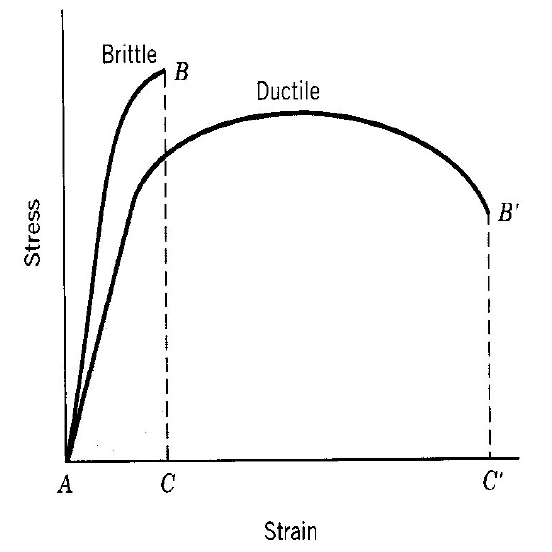
\includegraphics[width = 0.4\textwidth]{ProvaTrazione}} \quad
\subfloat[][\emph{Grafico prova di trazione con snervamento discontinuo}\label{fig:trazioneDiscontinua}]{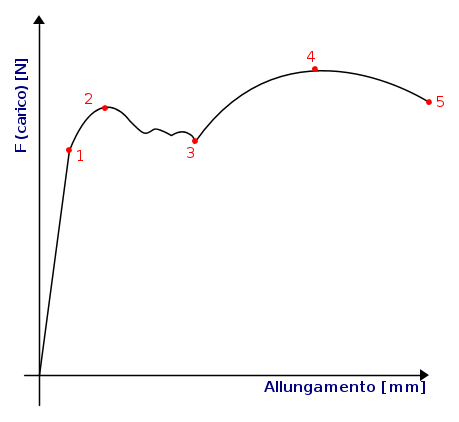
\includegraphics[width = 0.4\textwidth]{TrazioneDiscontinua}}
\caption{Prove di trazione}\label{fig:Trazione}
\end{figure}
Se si osserva il grafico della prova di trazione \ref{fig:TrazioneContinua}
si osservano 2 particolari zone: comportamento elastico del materiale e comportamento plastico.
Ricordando l'equazione constitutiva del materiale ovvero
\begin{equation}
\sigma = K \epsilon ^n
\label{eq:Cost}
\end{equation}
Dove i termini di \ref{eq:Cost} sono:\\
\begin{tabular}{cl}
$\sigma$ & tensione [MPa]\\
$K$ & coefficiente di resistenza\\
$\epsilon$ & fattore di incrudimento\\
$n$ & Sensibilità alla velocità di incrudimento\\
\end{tabular}
\\
Dalla \ref{eq:Cost} si può intuire che il il fattore $K$ lo si volgia particolarmente grande al fine di garantire un'alta resistenza allo snervamento.
La stizione si manifesterà su una sezione "più debole" (impurità, vuoti, ecc\dots), da cui avrà luogo una deformazione della sezione stessa. Dunque sulla sezione si manifesterà incrudimento dovuto proprio alla trasformazione.
L'incrudimento renderà la sezione molto più dura rispetto alle circostanti. Perciò si può dimostrare come il valore per cui la strizione si stabilizza è proprio pari al coefficiente $n$.
Sotto queste ipotesi allora vale:
\begin{equation}
\epsilon = n
\label{eq:StrizzCost}
\end{equation}
In generale si preferisce utilizzare materiali con coefficiente $n$ molto alto: per cui il materiale 
si deforma molto prima della strizione. Dunque è più \textbf{duttile}.

\subsection{Snervamento discontinuo}
Lo snervamento discontinuo è tipico dei metalli che hanno basso valore interstiziale.
Tipicamente, a fine lavorazione di tali metalli si presentano le \textbf{bande di Lüder}. Di fatto non costituiscono un difetto tecnologico, piuttosto puramente estetico. Siccome le lamiere vengono utilizzate anche per coperture, tali bande fanno sembrare il prodotto più scadente (Anche se di fatto non lo è).
Il grafico \ref{fig:trazioneDiscontinua} rappresenta il comportamento di un materiale a snervamento discontinuo.

\section{Tessitura e anisotropia}
La tessitura è la descrizione della presentazione, sia estetica che prestazionale, del materiale
Logicamente dipende direttamente dai grani cristallini presenti nel materiale.

Quando questi si presentano in forma allungata (es. post laminazione), portano 
a delle differenze dal punt odi vista meccanico-fisico del prodotto. 
Portando \textbf{anisotropia}.
Già si sa che i piani preferenziali di scorrimento sono quelli ad alte densità atomica
e, nel caso non ce ne siano a sufficienza, il materiale tenderà a costituirne di nuovi%
\footnote{Si vedrà anche in seguito che la questione dei piani di scorrimento è cruciale per la qualità del materiale}.

\subsection{Proprietà modificate}
Ricordando i principali termini di descrizione delle proprietà meccanico-fisiche dei metalli:\\
\begin{tabular}{cl}
$Y$ & Densità di snervamento\\
$T_S$& Resistenza meccanica\\
\end{tabular}
\\
Inoltre anche altre proprietà, non necessariamente meccaniche, vengono modificate da eventuali lavorazioni a freddo.
Allora: considerando una lamiera lavorata a freddo vale:
\begin{equation}
\epsilon_1 + \epsilon_2 + \epsilon_3 = 0 \underbrace{\rightarrow}_{\text{per lamiere}}
\epsilon_l + \epsilon_w + \epsilon_t = 0 
\label{eqn:DefCost}
\end{equation}
La \ref{eqn:DefCost} definisce la \emph{costanza della deformazione del volume principale}.
Si considerano pedici diversi da quelli classici per un volume massivo in quanto stiamo considerando una lamiera, percui i nuovi pedici indicano:\\
\begin{tabular}{cl}
$l$ & \textit{lenght}\\
$w$ & \textit{width}\\
$t$ & \textit{thickness}\\
\end{tabular}
\\
Si ricordano, inoltre, le deformazioni per le principali grandezze:
\begin{equation}
\epsilon_w = \ln{\frac{w_1}{w_0}} \qquad \epsilon_t = \ln{\frac{h_1}{h_0}}
\label{eqn:DefPrinc}
\end{equation}
Dove $w_1$ e $h_1$ sono le misurazioni dopo la prova di trazione, mentre $w_0$ e $h_0$ sono i valori iniziali.
A partire dai termini sopraelencati, si può definire il parametro $r$ definito come nella \ref{eqn:r}.
\begin{equation}
r = \frac{\epsilon_w}{\epsilon_t}
\label{eqn:r}
\end{equation}
Non ha un nome specifico, nonostante rappresenti la quantità di deformazione che una lamiera subisce se sottoposta a trazione.
In particolare, le due deformazioni considerate sono quella in termini di spessore e quella in larghezza.
Se il materiale avesse:
\begin{equation}
r = 1
\end{equation}
potrebbe essere considerato isotropo. Più correttamente si definiscono \textbf{isotropi} tutti quei materiali per cui vale la \ref{eqn:DefIsotropo}.
\begin{equation}
r_0 = r_{45} = r_{90} = 1
\label{eqn:DefIsotropo}
\end{equation}
dove i fattori $r$ sono il rapporto tra le deformazioni come sopra però ponendo la trazione con angolo tanto quando indicato dal pedice:\\
\begin{tabular}{cl}
$r_0$ & Direzione laminazione\\
$r_{45}$ & Direzione intermedia\\
$r_{90}$ & Direzione ortogonale
\end{tabular}
\\
Altrimenti il materiale è semplicemente \textbf{anisotropo}.
L'anisotropia può essere un problema in termini di lavorazione di una lamiera: si prenda come esempio il caso della realizzazione di un contenitore per estrusione. Se il materiale fosse isotropo allora la deformazione avverrebbe in maniera uniforme su tutta la lamiera.
Se, invece, il materiale è anisotropo, la deformazione diversificata produce variabilità sul bordo del prodotto. Successivamente sarebbe necessario un operazione di \textit{trimming} per eliminare il materiale in eccesso.
L'anisotropia si può verificare in diverse forme.
\begin{description}
\item[$r_0 = r_{45} = r_{90} \lessgtr 1$] allora si parla di \textbf{Anisotropia normale} alla superficie della lamiera. Se ne può misurare il valore tramite:
\begin{equation}
r_m = \overline{r} = \frac{r_0 + r_{90} + 2 * r_{45}}{4}
\label{eqn:MisAnisotropia}
\end{equation}
\item[$r_0 \neq r_{45} \neq r_{90}$] allora si parla di \textbf{compresenza di anisotropia planare e normale} da cui si può ottenere una misura
\begin{equation}
\Delta r = \frac{r_0 + r_{90} - 2 * r_{45}}{2}
\label{eqn:MisPlanare}
\end{equation}
\end{description}
In generale l'anisotropia si verifica quando, durante la laminazione, i reticoli cristallini si muovono per garantire i piani di scorrimento.
Ora si vuole dare una rapida visione delle principale strutture cristallini nei materiali.

\subsubsection{Reticolo esagonale compatto}
I piani di scorrimento si trovano sulle superfici di base del prisma compatto.
Si definisce \textit{compatto} perché il rapporto tra l'altezza del prisma e la lunghezza di un lato di base, ovvero $c/a$ considerando i riferimenti della figura \ref{fig:EsaComp}.
\begin{figure}
\centering
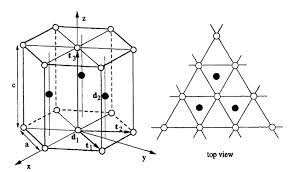
\includegraphics[width = 0.8\textwidth]{Esagono1}
\caption{Esagonale compatto}
\label{fig:EsaComp}
\end{figure}
Si osserva che il rapporto \ref{eqn:r} per materiali con reticolo cristallino \eng{High c/}a è prossimo a a 0:
\begin{equation}
r_{\text{High c/a}} = \frac{\epsilon_w}{\epsilon_t} \longrightarrow 0
\label{eqn:HighC_AR}
\end{equation}
Nella maggior parte dei casi si vuole un rapporto $r$ il più alto possibile. Così ché la deformazione della lamiera interessi la larghezza piuttosto dello spessore. Altrimenti potrebbero sorgere problemi sulla rigidità della lamiera anche senza eseguire alcuna lavorazione.
Potremmo allora dire che:
\begin{description}
\item[$n$] indichi il ritardo nella deformazione (sensibilità alla deformazione)
\item[$r$] indichi che tipo di deformazione si avrà. 
\end{description} 

Nel caso di materiali ad esagonale compatto ma con rapporto $c/a$ basso si osserva:
\begin{equation}
r_{\text{Low c/a}} \longrightarrow \infty 
\end{equation}
Ad esempio per guadagnare duttilità nel titanio (Ti) si effettuano lavorazioni a caldo.

\subsubsection{Reticolo cubico}
\begin{figure}
\centering
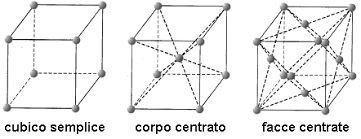
\includegraphics[width = \textwidth]{Cubico}
\caption{Reticoli cubici}
\label{fig:Cubici}
\end{figure}
Per i metalli cristallizzanti a \ac{CFC} si osserva un valore di $r\approx 0.4 \div 0.8$.
Mentre per i metalli a \ac{CCC} si osservano valori di $r \approx 1$.

\section{Effetti delle lavorazioni a freddo}
Come già accennato in precedenza, le lavorazioni a freddo permettono di ottenere da un materiale metallico sì la deformazione voluta. In più si garantisce al materiale maggiore durezza.
Ciò è dovuto allo scorrimento delle dislocazioni, durante la lavorazione del materiale, che vengono bloccate dal bordo del grano cristallino.
Di contro bisogna tenere a mente che una maggiore durezza impone una minore duttilità, considerazione che serve nel caso la lamiere debba subire diverse lavorazioni prima di divenire prodotto finito.
\missingfigure{Da aggiungere il grafico tridimensionale sulla deformazione a freddo.}
\missingfigure{Aggiungere proiezioni del grafico precedente in due dimensioni.}

Dunque le lavorazioni a freddo hanno diversi vantaggi e svantaggi come descritto nella tabella \ref{tab:VantSvantFreddo}.

\begin{table}
\centering
\caption{Vantaggi e svantaggi delle lavorazioni a freddo}
\label{tab:VantSvantFreddo}
\begin{tabularx}{\textwidth}{XX}
\toprule
\textcolor{UnifeDark}{\textbf{Vantaggi}} & \textcolor{UnifeDark}{\textbf{Svantaggi}}\\
\midrule
Metodo economico per indurire il materiale &
Pressione sugli stampi più alti\\
Il prodotto è quasi finito finite le lavorazioni (in genere) &
Bisogna trovare un compromesso tra durezza desiderata e consumo delle attrezzature\\
\bottomrule
\end{tabularx}
\end{table}

Per ovviare ad alcuni problemi evidenziati alla tabella \ref{tab:VantSvantFreddo}, si può pensare di ricorrere a ricotture parziali o complete.
Alcuni esempi sono riportati alle figure \ref{fig:RsRicottura}

In particolare:
\begin{description}
\item[Lavorazione a freddo $T < 0.3 T_m$] evidenzia un chiaro incrudimento del materiale, che ne risulterà indurito.
\item[Ricotture di distensione $0.3T_m < T < 0.5 T_m$] Permette una ridistribuzione delle dislocazioni ma senza ricristallizzazione
\item[Ricottura di ricristallizzazione $T > 0.5 T_m$] Non è scontata la ricristallizzazione ma si ha una distensione dei grani, annullando eventuali lavorazioni a freddo precedenti.
\end{description}
Nonostante ciò le ricotture possono essere molto interessanti per le caratteristiche meccaniche dei materiali metallici.
Ipotizzando di voler raggiungere un determinato obbiettivo di duttilità del materiale. Si può raggiungere tale obbiettivo semplicemente lavorando il materiale a freddo, dando una certa deformazione al pezzo.
Sappiamo che così il pezzo sarà più indurito di conseguenza.
C'è un ulteriore modo: se si incrudisce di più rispetto al obbiettivo, attraverso una deformazione maggiore di quella desiderata, si può pensare di sfruttare una ricottura di distensione per ritornare al livello di duttilità richiesto ma garantendo un livello di durezza maggiore rispetto alla sola lavorazione a freddo. In genere vale anche il viceversa. 
Tale metodo viene chiamato \textit{forte incrudimento con ricottura parziale}.
Alla figura \ref{fig:Ricot} è graficato l'andamento delle tensioni di snervamento e rottura dopo una ricottura completa. Si osserva che vengono perse completamente le caratteristiche meccaniche guadagnate tramite incrudimento per lavorazione a freddo.
Alla figura \ref{fig:RicotRs} viene mostrato il processo per ottenere una determinata tensione di snervamento dopo forte incrudimento. 

\begin{figure}
\centering
\subfloat[][\emph{Duttilità, snervamento e rottura dopo ricottura}\label{fig:Ricot}]%
{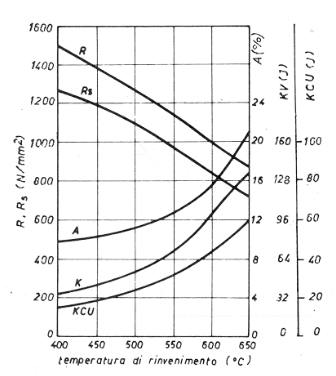
\includegraphics[width = 0.4\textwidth]{Rinvenimento}}\quad
\subfloat[][\emph{Durata ricottura in base allo snervamento richiesto}\label{fig:RicotRs}]%
{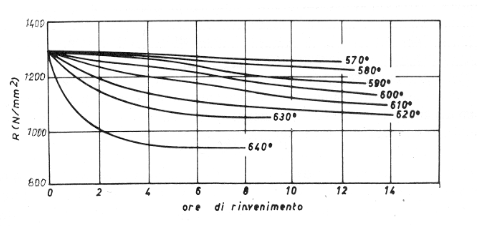
\includegraphics[width = 0.4\textwidth]{CotturaRinvenimento}}
\caption{Andamenti tipici di un acciaio dopo ricottura}\label{fig:RsRicottura}
\end{figure}

Ipotizzando una ricottura completa, ovvero portando il materiale a una temperatura $T > 0.5\:T_m$, si può avere ricristallizzazione del metallo che porta grani a dimensioni maggiori. Bisogna anche tenere a mente l'influenza del tempo su questi processi di ricottura.

\subsection{Effetti della velocità di deformazione}
Come visto nell'equazione costitutiva \ref{eqn:DefCost}, il materiale viene univocamente definito tramite tale equazione. In realtà è necessario "mettere in relazione" anche il tempo. Considerando l'equazione costitutiva per lavorazione a caldo:
\begin{equation}
\sigma_f = C \cdot \dot{\epsilon}^m
\label{eqn:CostCaldo}
\end{equation}
Da cui si può osservare che se la temperatura aumenta allora $C$ diminuisce e contemporaneamente $m$ cresce. Infatti:
\begin{description}
\item[$C$] è il coefficiente di resistenza alla temperatura del materiale;
\item[$m$] è l'indice di sensibilità alla velocità di deformazione;
\item[$\dot{\epsilon}$] è la velocità di deformazione descritta come $V/h$
\end{description}
Con una strizione diffusa, l'incrudimento è diffuso su tutto il provino. E, come si era visto anche in precedenza, ciò migliora le caratteristiche meccaniche. Se invece, la strizione è localizzata rischia di indebolire il materiale.
Il fatto che sia locale indica che il materiale in quel punto è più debole e può rompersi più facilmente.

\begin{definition}{Considerazione}{*}
In generale si privilegiano metalli che abbiano alta sensibilità al incrudimento e maggiore sensibilità alla velocità di strizionamento.
\end{definition}


Si vogliono ricordare i valori per cui $m$ porta ad un determinato comportamento il materiale:
\begin{description}
\item[$-0.05 < m < 0.05$] \eng{Cold working}
\item[$0.05 < m < 0.3$] \eng{Hot working}
\item[$0.3 < m < 0.7$] \eng{Superplasicity}%
\footnote{Valori di deformazione tipici delle lavorazioni con materiali plastici}
\item[$m > 1$] \eng{Newtonian fluid}
\end{description}

\section{Limiti di formabilità delle lamiere}
\begin{enumerate}
\item Manifestazione di strizioni localizzate.
\item Con strizione diffusa, prima della rottura.
\item Generazione delle bande di L\"uder
\item Generazione della superficie a buccia d'arancia
\end{enumerate}
A parte le prime due che portano a conseguenze meccaniche per cui la lamiera effettivamente non può più essere vendute o utilizzate per la produzione.
La terza ha una motivazione puramente estetica: siccome le lamiere possono essere utilizzate come copertura, tale superficie può essere problematica. Non lo è dal punto di vista meccanico-fisico.
La superficie a buccia d'arancia anch'essa non influisce sulle prestazione meccaniche del prodotto%
\footnote{C'è da dire che una maggiore porosità superficiale potrebbe stimolare la generazione di cricche in alcune lavorazioni.}.
La formazione è dovuta alla rotazione dei grani cristallini durante eventuali lavorazioni.
La soluzione è quella di sfruttare, per le lamiere in particolare, materiali a grana fine.

\subsection{Come mai le lamiere?}
Le lamiere vengono largamente impiegate largamente per la produzione di oggetti metallici, e le tecniche che verranno trattate in questo corso volgono a a sfruttare tale prodotti in larga scala.
\todo{\\Da rivedere :-/}
Principalmente le lamiere vengono sfruttate perché:
\begin{itemize}
\item A parità di prodotto, un oggetto pieno e uno ricavato tramite lavorazione di lamiera risulta più pesante.
\item La laminazione è una lavorazione molto efficiente: si producono tanti pezzi in poco tempo e con minore energia.
\item La laminazione permette di raggiungere risultati molto accurati (in termini di spessori e qualità del laminato) con poche risorse, dunque ad un costo molto basso.
\item La lamiera è un prodotto "quasi" pronto all'uso.
\end{itemize}

\section{Materiali per lamiere}
I materiali che in industria vengono più comunemente utilizzati per lamiere sono ad esempio:
\begin{itemize}
\item Acciai, dolci + inossidabili
\item Leghe di allumino
\item Ottoni
\item Bronzi
\item Rame
\item Magnesio
\item Titanio
\end{itemize}
Sebbene la maggior parte dei prodotti in lamiera siano lavorati a freddo, ci sono alcuni materiali che necessitano di lavorazioni a caldo.
In particolare alla figura \ref{fig:LavCaldo}, si presentano i motivi per cui sia necessaria la lavorazione a caldo

\begin{figure}
\centering
\usetikzlibrary{trees}
\begin{tikzpicture}[
sibling distance = 10em,
every node/.style={rectangle, rounded corners, draw, align=center}]
\node[top color=UnifeLight]{Lavorazioni a caldo}
	child{node[top color=UnifeDark, bottom color=UnifeDark!50, white]{Esagonale\\compatto}
		child{node[top color=UnifeDark!50, bottom color=UnifeDark!50, white]{Maggiore\\duttilità}}
		child{node[top color=UnifeDark!50, bottom color=UnifeDark!50, white]{Si spera in\\un cambio\\di reticolo}}}
	child{node[top color=UnifeDark, bottom color=UnifeDark!50, white]{Superplasticità}}
	child{node[top color=UnifeDark, bottom color=UnifeDark!50, white]{Forze troppo\\alte}};
\end{tikzpicture}
\caption{Motivazioni delle lavorazioni a caldo}
\label{fig:LavCaldo}
\end{figure}
Ora si vedranno nel dettaglio tutte le caratteristiche e motivazioni per cui viene scelta una determinata categoria di materiali.

\subsection{Acciai}
In genere si preferiscono acciai che abbiano un tenore di carbonio minore del 0.15\%, ovvero gli acciai dolci.
Inoltre, bisogna includere gli acciai inossidabili: sia per motivi di mercato, che necessità operative dei prodotti finali.
Essendo una gamma decisamente ampia di materiali, le lavorazioni possibili sono molteplici:
\begin{description}
\item[lavorazioni a caldo] non vengono sfruttate troppo per gli acciai in quanto si preferisce mantenere l'incrudimento ottenuto tramite la lavorazione a freddo. Anche se si impiega per:
	\begin{itemize}
	\item Ottenere maggiore duttilità per il materiale.
	\item Quando le forze in gioco sono eccessive è opportuno aumentare la duttilità grazie ad 
	una maggiore temperatura.
	\end{itemize}
	Si rischia di incorrere in:
	\begin{itemize}
	\item Finiture peggiori.
	\item Maggiore rugosità da cui derivano pure caratteristiche meccaniche peggiori.
	\item Non si ottiene incrudimento. 
	\end{itemize}
\item[Lavorazioni a freddo] In industria vengono sfruttate molto più volentieri per via:
	\begin{itemize}
	\item Migliori tolleranze geometriche ottenibili.
	\item Migliore finitura superficiale,
	\item Migliori prestazioni meccaniche a parità mi materiale usato.
	\end{itemize}
\end{description}

